\section{Сумма Минковского.  Задача планирования движения робота в среде с препятствиями. Граф видимости.}

\subsection{Граф видимости}

Рассмотрим точное решение нахождения кратчайшего пути на плоскости между двумя точками с полигональными препятствиями с помощью построения графа видимости.
После его построения кратчайший путь ищется любым стандартным алгоритмом поиска (например, алгоритмом Дейкстры или A*).

Для простоты рассуждений начальную и конечную вершины будем считать вершинами полигонов. 

\begin{lemma}
    Любой кратчайший путь между двумя вершинами с полигональными препятствиями представляет собой ломаную, вершины которой — вершины полигонов.
\end{lemma}
\begin{proof}
    Пусть кратчайший путь --- не ломаная.
    В таком случае, на пути существует такая точка $p$, которая не принадлежит ни одному прямому отрезку.
    Это означает, что существует $\varepsilon$-окрестность точки $p$, в которую не попадает ни одно препятствие (случай, когда точка попала на ребро рассматривается аналогично).
    В таком случае, подпуть, который находится внутри $\varepsilon$-окрестности, по неравенству треугольника может быть сокращён по хорде, соединяющий точки пересечения границы $\varepsilon$-окрестности с путем.
    Раз часть пути может быть уменьшена, значит и весь путь может быть уменьшен, а значит исходное предположение некорректно. 
\end{proof}

\begin{definition}
    Говорят, что вершина $u$ видна (англ. mutually visible) из $v$, если отрезок $uv$ не пересекает ни одного препятствия.
\end{definition}

\begin{definition}
    Граф видимости (англ. visibility graph) --- граф, вершины которого --- вершины полигонов.
    Между вершинами $u$ и $v$ существует ребро, если из $u$ видна v.
\end{definition}

В худшем случае в таком графе может быть $O(n^2)$ ребер.
Однако по некоторым ребрам кратчайший путь точно не пройдет, и такие ребра из графа можно удалить. 

\begin{lemma}
    \begin{enumerate}
        \item Если существуют вершины $A,B,C$ одного препятствия и вершина $D$ такая, что поворот $DBA$ не совпадает с поворотом $DBC$, то ребро $DB$ не принадлежит кратчайшему пути и его можно удалить из графа.
        \item Все внутренние вершины, кроме вырожденного случая, (начальная/конечная точка лежит внутри выпуклой оболочки фигуры) можно игнорировать.
    \end{enumerate}
\end{lemma}
\begin{proof}
    \begin{enumerate}
        \item Путь проходящий через ребро $BD$ будет длиннее, чем через соседей точки $B$, так как по неравенству треугольника $AB+BD>AD$.
        \item Если случай не вырожденный, значит заход внутрь фигуры только увеличит суммарный путь, так как по неравенству треугольника расстояние между соседними выпуклыми вершинами всегда меньше суммы расстояний с учётом внутренней.
    \end{enumerate}
\end{proof}

\begin{figure}
    \centering
    \includegraphics[width=0.5\linewidth]{images/15_2.png}
    \caption{Удаляем $BD$}
\end{figure}

\begin{figure}
    \centering
    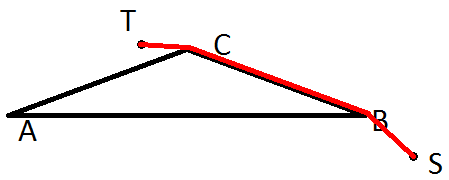
\includegraphics[width=0.5\linewidth]{images/15_3.png}
    \caption{Не удаляем $BS$}
\end{figure}

По доказанным леммам любое ребро кратчайшего пути содержится в графе.
Таким образом, для нахождения кратчайшего пути осталось найти кратчайший путь в этом графе от начальной до конечной вершины. 

\subsection{Планирование движения}

Рассмотрим задачу нахождения кратчайшего пути, когда движимый объект --- это выпуклый полигон.
Например, робот, которого надо доставить из начальной в конечную точку. 

Если полигон вращать нельзя, задачу сводится к движению точки так: выбирается точка на полигоне, которая принимается за начало координат.
В такой системе координат для каждого препятствия считается сумма Минковского с полигоном.
Получаются бОльшие препятствия, но теперь достаточно двигать выбранную точку, что было описано выше.

\subsection{Сумма Минковского}

Каждой точке $(x,y)$ ставится в соответствие фигура робота $R(x,y)$ с точкой привязки, помещенной в точку $(x,y)$.

\begin{definition}
    Для заданного робота $R$ и препятствия $P$, $К$-препятствием называется множество точек, будучи помещенным в которые, робот заденет препятствие: $CP:=\{(x,y):R(x,y) \cap P \not= \emptyset \}$.
\end{definition}

\begin{definition}
    Суммой Минковского двух множеств $S_1 \subset R^2$, $S_2 \subset R^2$ называется множество $S_1 \oplus S_2:=\{p+q:p \in S_1,q \in S_2\}$, где $p+q$ обозначает векторную сумму.
\end{definition}

\begin{definition}
    Отрицанием множества $S \subset R^2$ называется множество $-S:=\{−p:p \in S \}$, где $-p$ обозначает векторное отрицание.
\end{definition}

\begin{theorem}
    Для заданного робота $R$ и препятствия $P$, $К$-препятствием является множество $P \oplus (-R(0,0))$.
\end{theorem}
\begin{proof}
    Необходимо доказать, что робот $R(x,y)$ пересекает препятствие $P$ в том и только в том случае, если $(x,y) \in P \oplus (-R(0,0))$.
    
    Пусть робот задевает препятствие, и точка $q=(q_x,q_y)$ является точкой пересечения.
    Тогда, так как $q \in R(x,y)$, то $(q_x−x,q_y−y) \in R(0,0)$, или $(x−q_x,y−q_y) \in −R(0,0)$.
    А заметив, что $q \in P$, получаем $(x,y) \in P \oplus (-R(0,0))$.

    В обратную сторону, пусть $(x,y) \in P \oplus (-R(0,0))$, тогда существуют точки $(r_x,r_y) \in R(0,0)$ и $(p_x,p_y) \in P$ такие, что $(x,y)=(p_x−r_x,p_y−r_y)$ или $(p_x,p_y)=(x+r_x,y+r_y)$, а это означает, что $R(x,y)$ пересекает $P$. 
\end{proof}

\begin{theorem}
    Пусть заданы две выпуклые фигуры $P$ и $R$ с числом вершин $n$ и $m$ соответственно.
    Тогда суммой Минковского $P \oplus R$ является выпуклая фигура с не более чем $m+n$ вершинами.
\end{theorem}
\begin{proof}
    Для начала заметим, что любая крайняя точка в направлении вектора $\vec{d}$ есть сумма крайних точек фигур в этом направлении.
    Убедиться в этом можно, спроецировав обе фигуры на вектор $\vec{d}$.

    Теперь рассмотрим произвольное ребро $e$ из $P \oplus R$. 
    Оно является крайним в направлении к своей нормали, а значит оно образовано крайними точками фигур, и хотя бы у одной из фигур должно быть ребро, которое является крайним в этом направлении.
    Сопоставим $e$ с этим ребром.
    Тогда, сопоставив таким образом всем ребрам $P \oplus R$ ребра исходных фигур, получаем, что всего ребер в $P \oplus R$ не более чем $m+n$, так как каждое ребро исходных фигур использовалось не более раза. 
\end{proof}

\subsubsection{Псевдокод}

\begin{minted}{c}
 i = j = 0
 V[n] = V[0], V[n+1] = V[1], W[m] = W[0], W[m+1] = W[1]
 while i < n or j < m do
   add V[i]+W[j] to answer
   if angle(V[i], V[i+1]) < angle(W[j], W[j+1])
     ++i
   else if angle(V[i], V[i+1]) > angle(W[j], W[j+1])
     ++j
   else
     ++i, ++j
\end{minted}

\subsubsection{Случай невыпуклых фигур}

Для начала заметим следующий факт: $S_1 \oplus (S_2 \cup S_3)=(S_1 \oplus S_2) \cup (S_1 \oplus S_3)$.

В случае, когда одна из фигур невыпукла, её сначала надо затриангулировать, получив $n-2$треугольников.
После этого, уже известным алгоритмом, надо построить $n-2$ выпуклых фигур с не более чем $m+3$ вершинами, которые будут суммами Минковского соответствующих треугольников.
Объединение этих выпуклых фигур будет состоять из $O(nm)$ вершин.

В случае, когда обе фигуры невыпуклы, обе эти фигуры надо затриангулировать, получив $n-2$ и $m-2$ треугольников соответственно.
Построив суммы Минковского множеств этих треугольников, получим $(n-2)(m-2)$ выпуклых фигур, объединение которых состоит из $O(n^2m^2)$ вершин. 
